\documentclass[tikz,border=5mm]{standalone}
\usepackage{tikz}
\usepackage{eurosym}
\usetikzlibrary{positioning, shapes.geometric, shadows}

\begin{document}

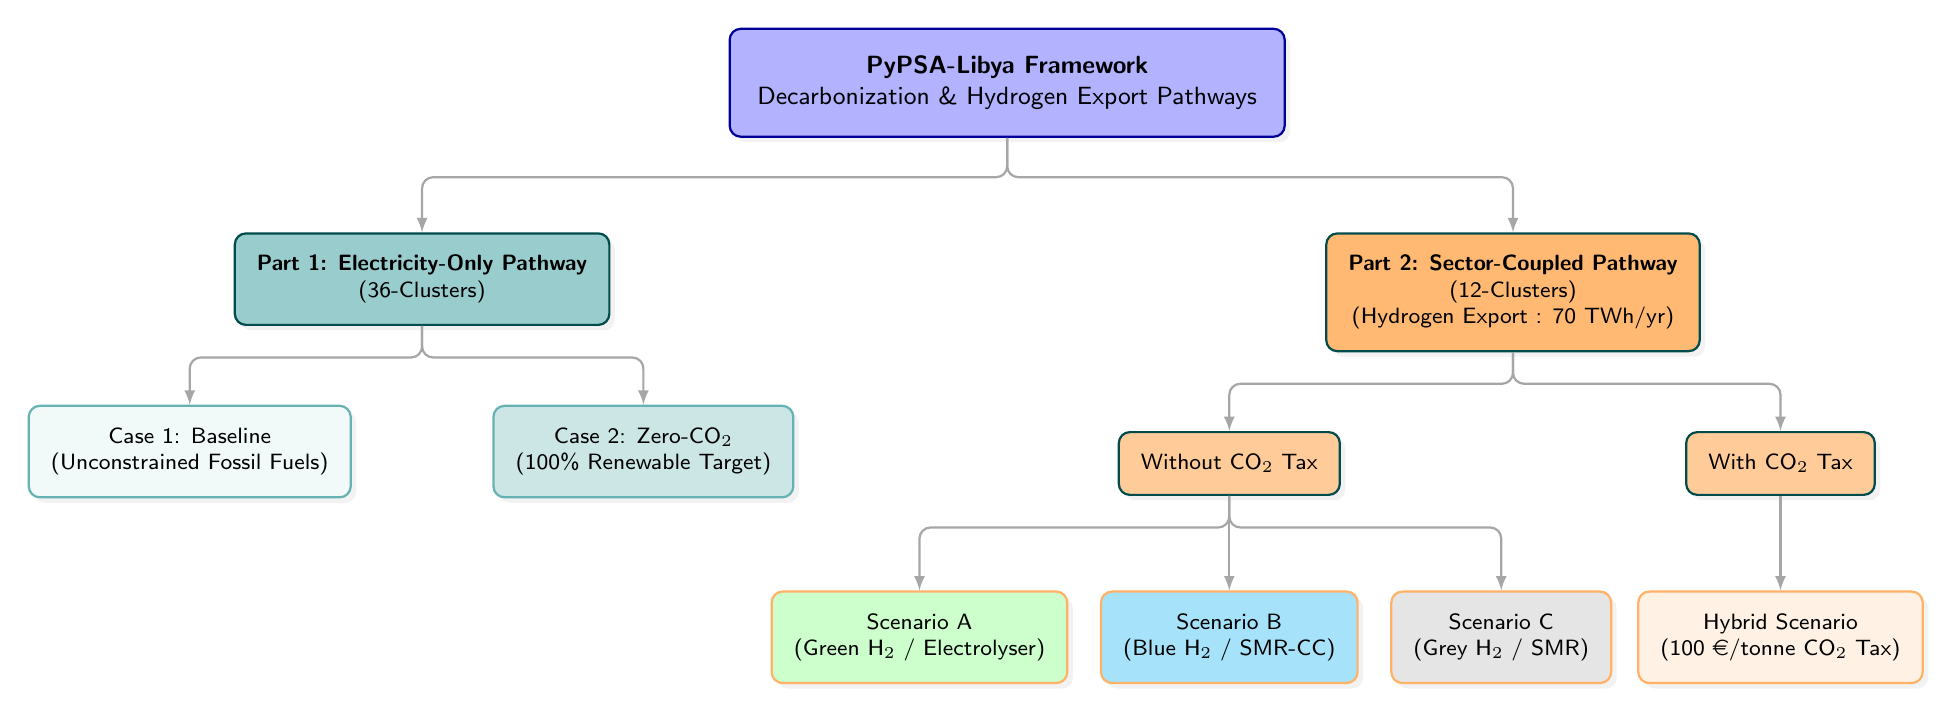
\begin{tikzpicture}[
    % Base node styling
    base/.style={
        draw=gray!60,
        thick,
        rectangle,
        rounded corners=4pt,
        align=center,
        inner sep=8pt,
        font=\sffamily\footnotesize,
        drop shadow={opacity=0.1, shadow xshift=2pt, shadow yshift=-2pt}
    },
    % Specific block stylings
    rootNode/.style={
        base,
        draw=blue!60!black,
        fill=blue!30,
        text=black,
        font=\sffamily\bfseries\small,
        inner sep=10pt
    },
    part1Header/.style={
        base,
        draw=teal!60!black,
        fill=teal!40,
        font=\sffamily\bfseries\footnotesize
    },
    part2Header/.style={
        base,
        draw=teal!60!black,
        fill=orange!55,
        font=\sffamily\bfseries\footnotesize
    },
    part3Header/.style={
        base,
        draw=teal!60!black,
        fill=orange!40,
    },
    caseNode1/.style={
        base,
        fill=teal!5,
        draw=teal!60
    },
    caseNode2/.style={
        base,
        fill=teal!20,
        draw=teal!60
    },
    scenNode/.style={
        base,
        fill=orange!20,
        draw=orange!30
    },
    scenNode_A/.style={
        base,
        fill=green!20,
        draw=orange!60
    },
    scenNode_B/.style={
        base,
        fill=cyan!35,
        draw=orange!60
    },
    scenNode_C/.style={
        base,
        fill=gray!20,
        draw=orange!60
    },
    hybridNode/.style={
        base,
        fill=orange!10,
        draw=orange!60
    },
    metricNode/.style={
        draw=gray!50,
        thick,
        dashed,
        rectangle,
        rounded corners=2pt,
        fill=gray!5,
        align=center,
        inner sep=8pt,
        font=\sffamily\footnotesize\itshape,
        drop shadow={opacity=0.05}
    },
    % Connector line styling
    connector/.style={
        draw=gray!70,
        -latex,
        thick,
        rounded corners=4pt
    }
]

% --- LEVEL 0: ROOT ---
\node[rootNode] (root) {PyPSA-Libya Framework \\ \mdseries  Decarbonization \& Hydrogen Export Pathways};

% --- LEVEL 1: PARTS (Balanced Spacing with normal font in parentheses) ---
\node[part1Header, below left=1.2cm and 1.5cm of root] (part1) {Part 1: Electricity-Only Pathway \\ \mdseries (36-Clusters)};
\node[part2Header, below right=1.2cm and 0.5cm of root] (part2) {Part 2: Sector-Coupled Pathway \\ \mdseries (12-Clusters) \\ \mdseries (Hydrogen Export : 70 TWh/yr)};

% --- LEVEL 2: CASES & SCENARIO TYPES ---
\node[caseNode1, below left=1.0cm and -1.5cm of part1] (case1) {Case 1: Baseline \\ (Unconstrained Fossil Fuels)};
\node[caseNode2, below right=1.0cm and -1.5cm of part1] (case2) {Case 2:  Zero-CO$_2$ \\ (100\% Renewable Target)};

\node[part3Header, below left=1.0cm and -0.2cm of part2] (baseline) {Without CO$_2$ Tax};
\node[part3Header, below right=1.0cm and -0.2cm of part2] (policy) {With CO$_2$ Tax};

% --- LEVEL 3: SCENARIOS ---
\node[scenNode_B, below=1.2cm of baseline] (scenB) {Scenario B \\ (Blue H$_2$ / SMR-CC)};
\node[scenNode_A, left=0.4cm of scenB] (scenA) {Scenario A \\ (Green H$_2$ / Electrolyser)};
\node[scenNode_C, right=0.4cm of scenB] (scenC) {Scenario C \\ (Grey H$_2$ / SMR)};

\node[hybridNode, below=1.2cm of policy] (hybrid) {Hybrid Scenario \\ (100 \euro/tonne CO$_2$ Tax)};


% --- CONNECTIONS (ELBOW ROUTING) ---

% Root to Parts
\draw[connector] (root.south) -- ++(0,-0.5) -| (part1.north);
\draw[connector] (root.south) -- ++(0,-0.5) -| (part2.north);

% Part 1 to Cases
\draw[connector] (part1.south) -- ++(0,-0.4) -| (case1.north);
\draw[connector] (part1.south) -- ++(0,-0.4) -| (case2.north);

% Part 2 to Sub-branches
\draw[connector] (part2.south) -- ++(0,-0.4) -| (baseline.north);
\draw[connector] (part2.south) -- ++(0,-0.4) -| (policy.north);

% Baseline to Scenarios A, B, C
\draw[connector] (baseline.south) -- ++(0,-0.4) -| (scenA.north);
\draw[connector] (baseline.south) -- (scenB.north);
\draw[connector] (baseline.south) -- ++(0,-0.4) -| (scenC.north);

% Policy to Hybrid
\draw[connector] (policy.south) -- (hybrid.north);

\end{tikzpicture}
\end{document}